\documentclass[12pt,addpoints]{evalua}
\grado{2$^\circ$ de Secundaria}
\cicloescolar{2024-2025}
\materia{Ciencias y Tecnología: Física}
\unidad{2}
\title{Examen de {\color{brown}recuperación} de la Unidad}
\aprendizajes{\footnotesize%
      \item Comprende los conceptos de velocidad y aceleración.
      \item Describe, representa y experimenta la fuerza como la interacción entre
      objetos y reconoce distintos tipos de fuerza. Identifica y describe la presencia de fuerzas en interacciones
      cotidianas (fricción, flotación, fuerzas en equilibrio).
      \item Analiza la gravitación, las leyes de Newton y su papel en
      la explicación del movimiento de los
      planetas y en la caída de los cuerpos
      (atracción) en la superficie terrestre.
}
\author{Prof.: Julio César Melchor Pinto}
\begin{document}
\begin{multicols}{2}
      \include*{../blocks/block001}
      \include*{../blocks/block003}
      \include*{../blocks/block000}
      \include*{../blocks/block002}
\end{multicols}
\begin{questions}
      % \question[6]{Analiza el siguiente problema y selecciona la respuesta correcta para cada una de las preguntas:

      %       \begin{bA}
      %             En el beisbol el pitcher es el jugador encargado de lanzar la pelota a la posición del bateador del equipo contrario. Cada año, los pitcher de las Grandes Ligas intentan batir el récord mundial de velocidad de lanzamiento, que en el año 2006 pertenecía a Joel Zumaya, con una marca de 46.9 m/s. Cuatro años más tarde,  Neftali Feliz colocó la bola a 20 m del montículo en 0.43 segundos, y el ``Misil Cubano'', Aroldis Chapman, lo hizo en 0.42 segundos.
      %       \end{bA}

      %       \begin{parts}
      %             \part ¿Con qué rapidez viajó la bola que lanzó Neftali Feliz?

      %             \begin{oneparchoices}\footnotesize%
      %                   \choice 45.6 m/s  \choice 47.6 m/s \CorrectChoice 46. 5 m/s \choice 43. 5 m/s
      %             \end{oneparchoices}

      %             \part ¿Qué rapidez alcanzó la bola de Aroldis Chapman?

      %             \begin{oneparchoices}\footnotesize%
      %                   \choice 46.7 m/s  \choice 46.5 m/s \choice 47.3 m/s \CorrectChoice 47.6 m/s
      %             \end{oneparchoices}

      %             \part ¿De quién fue el lanzamiento más rápido?, ¿Por qué?

      %             \begin{choices}\footnotesize%
      %                   \choice El de Joel Zumaya, porque recorrió la misma distancia que los otros dos lanzamientos, pero en un menor tiempo. \CorrectChoice El de Aroldis Chapman, porque su lanzamiento recorrió la misma distancia en la menor cantidad de tiempo. \choice El de Neftali Feliz, porque recorrió la misma distancia en menor tiempo. \choice El lanzamiento de Neftali Feliz, porque recorrió la misma distancia en mayor tiempo.
      %             \end{choices}
      %       \end{parts}
      % }
      \newpage
      \question[8]{Analiza el siguiente problema y selecciona la respuesta correcta para cada una de las preguntas:

            \begin{bA}
                  Las 24 Horas de Le Mans es una competencia automovilística disputada en el Circuito de la Sarthe, en Le Mans, Francia; es la carrera de resistencia más peligrosa y cruel del mundo: el ganador es el piloto que recorre la mayor distancia en 24 horas. En 1966, Bruce McLaren, Ken Miles y Ronnie Bucknum, miembros de la misma escudería, cruzaron juntos la meta pero no todos dieron las mismas vueltas al circuito, y por lo tanto recorrieron diferentes distancias: 4 906.46 km, 4 906.44 km, y 4 743.2 km, respectivamente.
            \end{bA}

            \begin{parts}
                  \part ¿Cuál fue la rapidez media de Bruce McLaren?

                  \begin{oneparchoices}
                        \CorrectChoice 204.436 km/h
                        \choice 204.430 km/h
                        \choice 197.63 km/h
                        \choice 202.435 km/h
                  \end{oneparchoices}

                  \part ¿Qué rapidez media tuvo Ken Miles?

                  \begin{oneparchoices}
                        \choice 204.433 km/h
                        \choice 203.436 km/h
                        \CorrectChoice 204.435 km/h
                        \choice 197.63 km/h
                  \end{oneparchoices}

                  \part ¿Con qué rapidez viajó Ronnie Bucknum?

                  \begin{oneparchoices}
                        \choice 204.435 km/h
                        \CorrectChoice 197.63 km/h
                        \choice 204.436 km/h
                        \choice 195.63 km/h
                  \end{oneparchoices}

                  \part ¿Quién fue el más rápido?, ¿Por qué?

                  \begin{oneparchoices}
                        \choice  Bonnie Bucknun, porque recorrió la menor distancia en la misma cantidad de tiempo.
                        \CorrectChoice Bruce McLaren porque recorrió la mayor distancia en la misma cantidad de tiempo.
                        \choice Fueron igual de rápidos.
                        \choice Ken Miles, porque recorrió una gran distancia en la misma cantidad de tiempo.
                  \end{oneparchoices}
            \end{parts}
      }


      \question[12]{Analiza el siguiente problema y responde las preguntas:

            \begin{bA}
                  Una cantidad muy importante en el análisis de la “bioingeniería animal” es el número de unidades de longitud de su propio cuerpo que un animal recorre en un segundo.
                  El guepardo, considerado el animal terrestre más veloz del planeta, puede alcanzar una rapidez de 26.7 m/s. Mide 1.3 m, por tanto, se desplaza 20.5 longitudes de su cuerpo por segundo.
                  Por otro lado, el colibrí mide 0.10 m y se mueve a razón de 27.3 m/s, y un ácaro viaja a 0.322 m/s y sólo mide 0.001 m.
            \end{bA}

            \begin{parts}\setlength{\columnsep}{3em}
                  \begin{multicols}{2}
                        \part ¿Cuántas unidades de longitud de su propio cuerpo recorre el colibrí en un segundo?
                        % \begin{oneparchoices}
                        %      \CorrectChoice 273 cuerpos/s \choice 263 cuerpos/s \choice 20.5 cuerpos/s \choice 322 cuerpos/s
                        % \end{oneparchoices}

                        \begin{solutionbox}{5cm}\footnotesize%
                              Para obtener la rapidez del colibr\'i en $cuerpos/s$ a partir de la rapidez $v_c = 27.3$ en $m/s$ se debe
                              considerar la equivalencia entre la unidad de medida est\'andar (metro) y la longitud del colibr\'i (cuerpos):
                              \begin{align*}
                                    1 \text{ cuerpo}   & =  0.1 m                            \\
                                    \Rightarrow
                                    10 \text{ cuerpos} & = 1 m                               \\
                                    \therefore
                                    v_c                & = 27.3 \cdot (10 \text{ cuerpos})/s \\
                                    v_c                & = 273  \text{ cuerpos}/s
                              \end{align*}
                              El colibr\'i recorre 273 unidades de longitud de su propio cuerpo por cada segundo.
                        \end{solutionbox}

                        \part  ¿Cuál es la rapidez corporal del ácaro?
                        % \begin{oneparchoices}
                        %      \choice 273 cuerpos/s \CorrectChoice 322 cuerpos/s \choice 20.5 cuerpos/s \choice 324 cuerpos/s
                        % \end{oneparchoices}

                        \begin{solutionbox}{5cm}\footnotesize%
                              Para obtener la rapidez del \'acaro en $cuerpos/s$ a partir de la rapidez $v_a = 0.322$ en $m/s$ se debe
                              considerar la equivalencia entre la unidad de medida est\'andar (metro) y la longitud del \'acaro (cuerpos):
                              \begin{align*}
                                    1 \text{ cuerpo}      & =  0.001 m                              \\
                                    \Rightarrow
                                    1,000 \text{ cuerpos} & = 1 m                                   \\
                                    \therefore
                                    v_c                   & = 0.322 \cdot (1,000 \text{ cuerpos})/s \\
                                    v_c                   & = 322  \text{ cuerpos}/s
                              \end{align*}
                              El \'acaro recorre 322 unidades de longitud de su propio cuerpo por cada segundo transcurrido.
                        \end{solutionbox}
                  \end{multicols}

                  \part ¿Cuál de estos animales es el más rápido en relación con su tamaño corporal?, ¿Por qué?
                  % \begin{choices}
                  %      \choice El guepardo, porque recorre 20.5 longitudes de su cuerpo en tan solo un segundo. \CorrectChoice El ácaro, porque recorre el mayor número de unidades de longitud de su cuerpo en un segundo El colibrí, porque recorre el mayor número de unidades de longitud de su cuerpo en un segundo. \choice  Todos viajan con la misma rapidez, porque recorren la misma cantidad de longitudes de su cuerpo en un segundo.
                  % \end{choices}

                  \begin{solutionbox}{1.2cm}\footnotesize%
                        El \'acaro, ya que su rapidez en cuerpos/s es mayor, segun los resultados de los incisos anteriores.
                  \end{solutionbox}
            \end{parts}
      }

      \newpage

      % \question[5]{\include*{../questions/question033}}




      \question[10]{Elige la respuesta para cada pregunta, a partir de las imágenes de la figura \ref{fig:camionesdecarga01}.

            \begin{multicols}{2}
                  \begin{figure}[H]
                        \centering
                        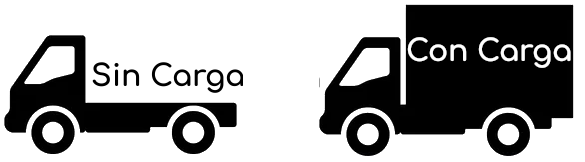
\includegraphics[width=0.8\linewidth]{../images/camionesdecarga01}
                        \label{fig:camionesdecarga01}
                        \caption{Representación de dos vehículos de carga.}
                  \end{figure}

                  \begin{parts}
                        \part  ¿Cuál de ellos será más difícil poner en movimiento?

                        \begin{checkboxes}
                              \choice El camión sin carga.
                              \CorrectChoice El camión cargado.
                              \choice Los dos camiones requieren el mismo esfuerzo.
                        \end{checkboxes}

                        \part  Si ambos camiones se movieran a la misma velocidad,
                        ¿a cuál de ellos le resultaría más fácil frenar?

                        \begin{checkboxes}
                              \choice El camión cargado.
                              \CorrectChoice El camión sin carga.
                              \choice Los dos camiones requieren el mismo esfuerzo.
                        \end{checkboxes}

                        \part  ¿Cuál podría aumentar más rápido su velocidad?

                        \begin{checkboxes}
                              \choice El camión cargado.
                              \CorrectChoice El camión sin carga.
                              \choice Los dos camiones aumentan su velocidad con la misma
                              rapidez.
                        \end{checkboxes}

                        \part  ¿Cuál de los camiones podría tomar una curva con más
                        facilidad si ambos se están moviendo a la misma velocidad?

                        \begin{checkboxes}
                              \CorrectChoice El camión sin carga.
                              \choice El camión cargado.
                              \choice Los dos camiones requieren el mismo esfuerzo.
                        \end{checkboxes}

                        \part ¿Cuál de ellos será más fácil poner en movimiento?
                        \begin{checkboxes}
                              \CorrectChoice El camión sin carga.
                              \choice El camión cargado.
                              \choice Los dos camiones requieren el mismo esfuerzo.
                        \end{checkboxes}

                        \part ¿Cuál podría aumentar más lento su velocidad?

                        \begin{checkboxes}
                              \choice El camión sin carga.
                              \CorrectChoice El camión cargado.
                              \choice Los dos camiones aumentan su velocidad con la misma rapidez.
                        \end{checkboxes}

                        \part Si ambos camiones se movieran a la misma velocidad,
                        ¿a cuál de ellos le resultaría más difícil frenar?

                        \begin{checkboxes}
                              \choice El camión sin carga.
                              \CorrectChoice El camión cargado.
                              \choice Los dos camiones requieren el mismo esfuerzo.
                        \end{checkboxes}

                        \part ¿Cuál de los camiones podría tomar una curva con más
                        dificultad si ambos se están moviendo a la misma velocidad?

                        \begin{checkboxes}
                              \CorrectChoice El camión sin carga.
                              \choice El camión cargado.
                              \choice Los dos camiones requieren el mismo esfuerzo.
                        \end{checkboxes}

                        \part Si se reduce la carga de arena de tal manera que la masa
                        del camión sea la mitad de su masa inicial, mientras el conductor pisa el
                        acelerador con la misma fuerza y mantiene el camión en la misma dirección,
                        ¿qué pasa con la acelaración del camión?

                        \begin{checkboxes}
                              \CorrectChoice Aumenta al doble.
                              \choice Disminuye a la mitad.
                              \choice No cambia.
                        \end{checkboxes}
                        %\vspace{1cm}

                        \part  Si el camión cargado va dejando gradualmente parte de su
                        cargamento mientras el
                        conductor pisa el acelerador con la misma fuerza y mantiene el camión
                        en la misma dirección,
                        ¿qué pasa con su rapidez?

                        \begin{checkboxes}
                              \CorrectChoice Aumenta.
                              \choice Disminuye.
                              \choice No cambia.
                        \end{checkboxes}
                  \end{parts}
            \end{multicols}
      }

      \question[5]{¿Qué fuerza se debe aplicar a una caja de 976 N de peso para subirla a un templete a una altura de 80 cm si se usa una rampa de 560 cm?

            \begin{solutionbox}{2cm}\footnotesize%
                  de la ecuación del plano inclinado se tiene:
                  \[F_1 \times d_1= F_2 \times d_2\]
                  donde $F_1=100$ N, $d_1=0.8$ m, $d_2=2.40$ m
                  $\Rightarrow$
                  \[
                        \begin{array}{lr}
                              100 \times 0.8              & = 	       F_2 \times 2.40
                              \\
                              \dfrac{100 \times 0.8}{2.4} & =  F_2
                              \\
                              \dfrac{100}{5}              & = 	      F_2
                              \\
                              20 = F_2
                        \end{array}
                  \]
            \end{solutionbox}
      }


      \question[12]{Analiza el siguiente problema y selecciona la respuesta correcta para cada una de las preguntas:
            \begin{bA}
                  Un mono trepa de manera vertical. Su movimiento se muestra en la siguiente gráfica (Fig. \ref{fig:dist_tiempo_03}) de la posición vertical, $y$, en funci\'on del tiempo, $t$.
            \end{bA}

            \begin{minipage}{0.3\textwidth}
                  \begin{figure}[H]
                        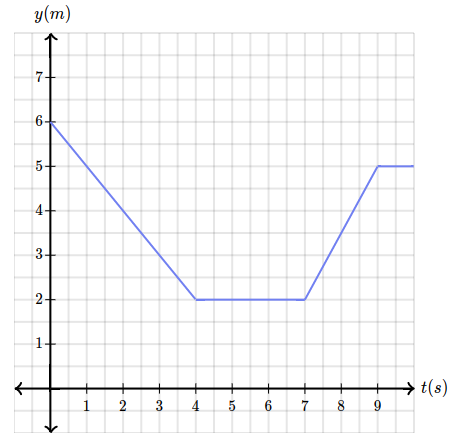
\includegraphics[width=1.25\linewidth]{dist_tiempo_03}
                        \caption{La gráfica representa el movimiento del mono.}%
                        \label{fig:dist_tiempo_03}
                  \end{figure}
            \end{minipage}\hfill%
            \begin{minipage}{0.6\textwidth}
                  \begin{parts}
                        \part  ¿Cuál es la rapidez instantánea del mono en $t=5\text{ s}$?

                        \begin{oneparcheckboxes}
                              \choice $5 \text{ m/s}$
                              \CorrectChoice $0 \text{ m/s}$
                              \choice $2.5 \text{ m/s}$
                              \choice $0.4 \text{ m/s}$
                        \end{oneparcheckboxes}

                        % \begin{minipage}{0.5\linewidth}

                        % \end{minipage}\hfill%
                        % \begin{minipage}{0.4\linewidth}
                        %       \ifprintanswers{\begin{solutionbox}{3cm}
                        %                   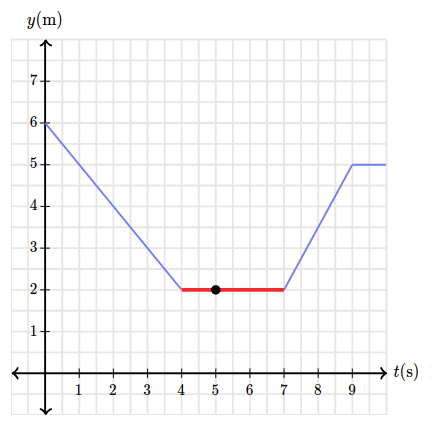
\includegraphics[width=\linewidth]{dist_tiempo_03c}
                        %             \end{solutionbox}}\else{}\fi
                        % \end{minipage}


                        \part  ¿Cuál es la velocidad instantánea del mono en  $t=8\text{ s}$?

                        \begin{oneparcheckboxes}
                              \CorrectChoice $1.5 \text{ m/s}$
                              \choice $0.42 \text{ m/s}$
                              \choice $2 \text{ m/s}$
                              \choice $1 \text{ m/s}$
                        \end{oneparcheckboxes}

                        % \begin{minipage}{0.5\linewidth}

                        % \end{minipage}\hfill%
                        % \begin{minipage}{0.4\linewidth}
                        %       \ifprintanswers{ \begin{solutionbox}{3cm}
                        %                   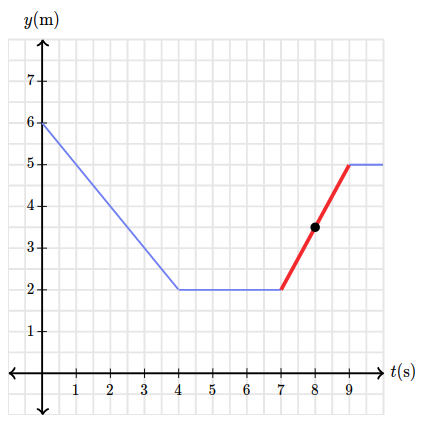
\includegraphics[width=\linewidth]{dist_tiempo_03b}
                        %             \end{solutionbox}}\else{}\fi
                        % \end{minipage}

                        % \part  ¿Cuál es la rapidez instantánea del mono en $t=6\text{ s}$?

                        % \begin{oneparcheckboxes}
                        %      \choice $5 \text{ m/s}$
                        %      \CorrectChoice $0 \text{ m/s}$
                        %      \choice $2.5 \text{ m/s}$
                        %      \choice $0.4 \text{ m/s}$
                        % \end{oneparcheckboxes}

                        % \columnbreak%

                        \part  ¿Cuál es la rapidez instantánea del mono en $t=2\text{ s}$?

                        \begin{oneparcheckboxes}
                              \choice $1 \text{ m/s}$
                              \choice $2 \text{ m/s}$
                              \CorrectChoice $-1 \text{ m/s}$
                              \choice $-2 \text{ m/s}$
                        \end{oneparcheckboxes}

                        % \begin{minipage}{0.5\linewidth}

                        % \end{minipage}\hfill%
                        % \begin{minipage}{0.4\linewidth}
                        %       \ifprintanswers{ \begin{solutionbox}{3cm}
                        %                   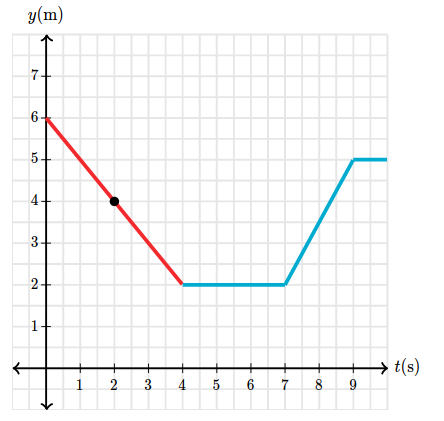
\includegraphics[width=\linewidth]{dist_tiempo_03a}
                        %             \end{solutionbox}}\else{}\fi
                        % \end{minipage}

                        \part ¿Cuál es la rapidez promedio del mono $t=4\text{ s}$ y $t=10\text{ s}$?

                        \begin{oneparcheckboxes}
                              \choice $ 1.5 \text{ m/s}$
                              \CorrectChoice $ 0.5 \text{ m/s}$
                              \choice $ 0 \text{ m/s}$
                              \choice $ -0.5 \text{ m/s}$
                        \end{oneparcheckboxes}

                        % \begin{minipage}{0.5\linewidth}

                        % \end{minipage}\hfill%
                        % \begin{minipage}{0.4\linewidth}
                        %       \ifprintanswers{\begin{solutionbox}{3cm}
                        %                   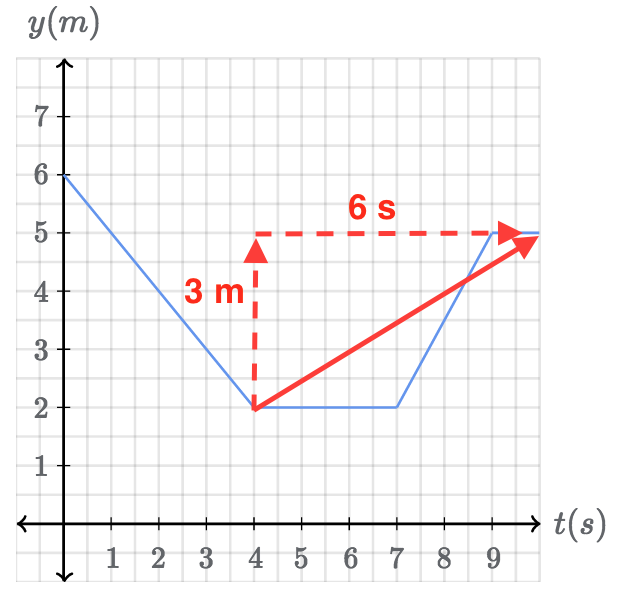
\includegraphics[width=\linewidth]{dist_tiempo_03d}
                        %             \end{solutionbox}}\else{}\fi
                        % \end{minipage}

                        \part  ¿Cuál es la rapidez promedio del mono $t=0\text{ s}$ y $t=7\text{ s}$?

                        \begin{oneparcheckboxes}
                              \CorrectChoice $ 0.5 \text{ m/s}$
                              \choice $ 1.5 \text{ m/s}$
                              \choice $ 0 \text{ m/s}$
                              \choice $ -0.5 \text{ m/s}$
                        \end{oneparcheckboxes}

                        % \begin{minipage}{0.5\linewidth}

                        % \end{minipage}\hfill%
                        % \begin{minipage}{0.4\linewidth}
                        %       \ifprintanswers{\begin{solutionbox}{3cm}
                        %                   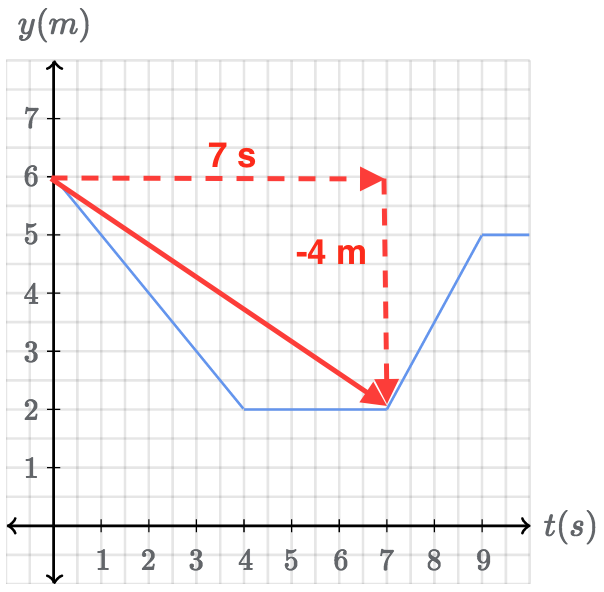
\includegraphics[width=\linewidth]{dist_tiempo_03e}
                        %             \end{solutionbox}}\else{}\fi
                        % \end{minipage}

                        \part  ¿Cuál es la rapidez promedio del mono $t=0\text{ s}$ y $t=10\text{ s}$?

                        \begin{oneparcheckboxes}
                              \CorrectChoice $ -0.1 \text{ m/s}$
                              \choice $ 1.5 \text{ m/s}$
                              \choice $ 0 \text{ m/s}$
                              \choice $ -0.5 \text{ m/s}$
                        \end{oneparcheckboxes}

                        % \begin{minipage}{0.5\linewidth}

                        % \end{minipage}\hfill%
                        % \begin{minipage}{0.4\linewidth}
                        %       \ifprintanswers{\begin{solutionbox}{3cm}
                        %                   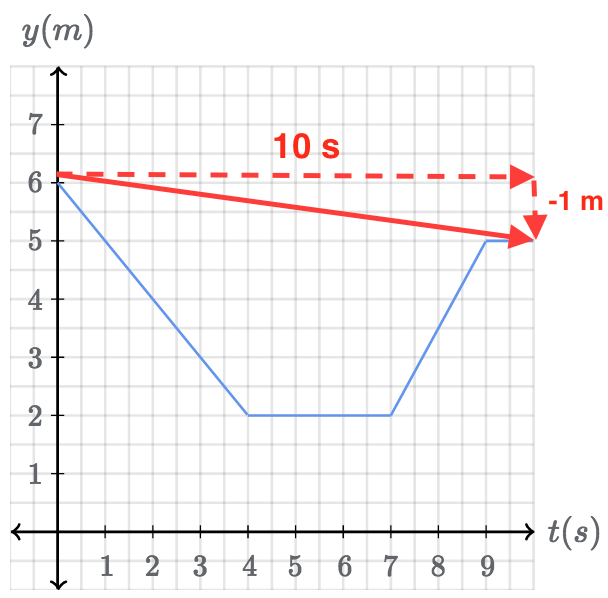
\includegraphics[width=\linewidth]{dist_tiempo_03f}
                        %             \end{solutionbox}}\else{}\fi
                        % \end{minipage}

                        % \part  ¿Cuál es la rapidez promedio del mono $t=4\text{ s}$ y $t=7\text{ s}$?

                        % \begin{oneparcheckboxes}
                        %      \choice $ -0.67 \text{ m/s}$
                        %      \choice $ 1.5 \text{ m/s}$
                        %      \choice $ 0.67 \text{ m/s}$
                        %      \CorrectChoice $ 0 \text{ m/s}$
                        % \end{oneparcheckboxes}
                  \end{parts}
            \end{minipage}
      }

      % \question[4]{Completa las afirmaciones de acuerdo con la información que presenta la gráfica de la figrua \ref{fig:dist_tiempo_01}.

      %       \begin{minipage}[t]{0.35\linewidth}
      %             \begin{figure}[H]
      %                   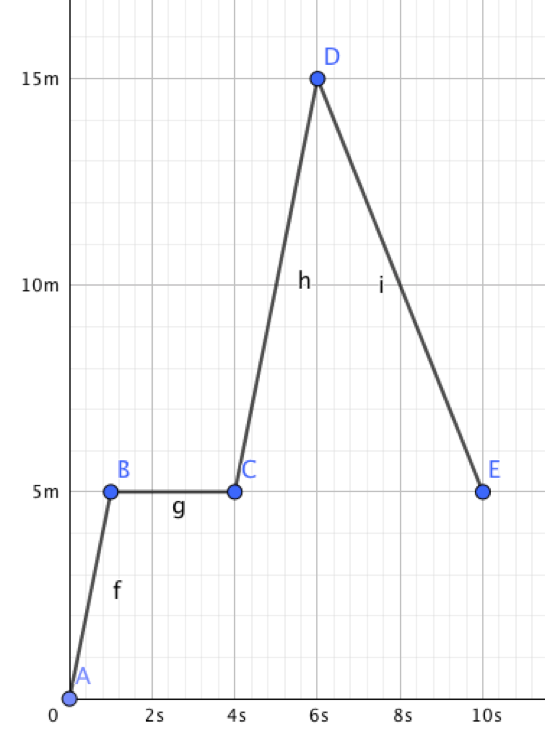
\includegraphics[width=\linewidth]{dist_tiempo_01}
      %                   \caption{La gráfica representa el desplazamiento de un atleta durante su entrenamiento.}
      %                   \label{fig:dist_tiempo_01}
      %             \end{figure}
      %       \end{minipage}%
      %       \begin{minipage}[t]{0.65\linewidth}
      %             \begin{parts}
      %                   \part  Después del primer esfuerzo, el atleta permaneció en reposo durante \fillin[3] segundos.

      %                   \part  La distancia total recorrida fue de \fillin[25] metros.

      %                   \part ¿Cu\'al fue la magnitud de la velocidad media durante el primer segundo de entrenamiento?

      %                   \begin{solutionbox}{3.5cm}\footnotesize%
      %                         La velocidad media durante el primer segundo de entrenamiento (punto B) de calcula tomando la distancia recorrida ($d=5$ m) dividido entre el tiempo $t=1$ s de recorrido:
      %                         \begin{align*}
      %                               v & =\frac{d}{t}                                 \\
      %                                 & =\frac{5\text{ m}}{1\text{s}} =5 \text{ m/s}
      %                         \end{align*}
      %                   \end{solutionbox}

      %                   \part ¿Cu\'al fue la magnitud de la velocidad media durante los primeros 6 segundos de entrenamiento?

      %                   \begin{solutionbox}{3.5cm}\footnotesize%
      %                         La velocidad media durante los primeros 6 segundos de entrenamiento (punto A al punto D) se calcula
      %                         tomando la distancia recorrida del punto A al punto D ($15$ m) dividido entre el tiempo $t=6$ s de recorrido:
      %                         \begin{align*}
      %                               v & =\frac{d}{t}                                   \\
      %                                 & =\frac{15\text{ m}}{6\text{s}} =2.5\text{ m/s}
      %                         \end{align*}
      %                   \end{solutionbox}



      %             \end{parts}
      %       \end{minipage}
      % }

      \question[10]{Señala si son verdaderas o falsas las siguientes afirmaciones:
            \begin{multicols}{2}
                  \begin{parts}
                        \part La velocidad y la rapidez se miden en unidades distintas.

                        \begin{oneparcheckboxes}
                              \choice Verdadero \CorrectChoice Falso
                        \end{oneparcheckboxes}
                        \part No es lo mismo desplazamiento que trayectoria.

                        \begin{oneparcheckboxes}
                              \CorrectChoice Verdadero \choice Falso
                        \end{oneparcheckboxes}
                        \part La rapidez tiene magnitud y direcci\'on.

                        \begin{oneparcheckboxes}
                              \choice Verdadero \CorrectChoice Falso
                        \end{oneparcheckboxes}
                        \part La rapidez es el cociente de la distancia recorrida por un objeto y el tiempo que tarda en recorrerla.

                        \begin{oneparcheckboxes}
                              \CorrectChoice Verdadero \choice Falso
                        \end{oneparcheckboxes}
                        \part La rapidez es el movimiento a gran velocidad.

                        \begin{oneparcheckboxes}
                              \choice Verdadero \CorrectChoice Falso
                        \end{oneparcheckboxes}
                        \part La distancia siempre es una cantidad positiva.

                        \begin{oneparcheckboxes}
                              \CorrectChoice Verdadero \choice Falso
                        \end{oneparcheckboxes}
                        \part En la aceleración se recorren distancias iguales en tiempos iguales.

                        \begin{oneparcheckboxes}
                              \choice Verdadero \CorrectChoice Falso
                        \end{oneparcheckboxes}
                        \part La aceleración es el cambio en el valor de la velocidad.

                        \begin{oneparcheckboxes}
                              \choice Verdadero \CorrectChoice Falso
                        \end{oneparcheckboxes}
                        \part La aceleración es una variable cinemática.

                        \begin{oneparcheckboxes}
                              \CorrectChoice Verdadero \choice Falso
                        \end{oneparcheckboxes}
                        \part La aceleración se mide en las mismas unidades que la velocidad.

                        \begin{oneparcheckboxes}
                              \choice Verdadero \CorrectChoice Falso
                        \end{oneparcheckboxes}
                  \end{parts}
            \end{multicols}
      }

      \newpage
      \question[16]{Analiza el siguiente problema y selecciona la respuesta correcta para cada una de las preguntas:
            \begin{bA}
                  Todas las mañanas Montse y Ricardo se desplazan de sus casas a la escuela.
                  A ella le gusta caminar y Ricardo utiliza su bicicleta.
                  En la gráfica de la Fig. \ref{fig:dist_tiempo_02} se representan sus movimientos.
            \end{bA}

            \begin{multicols}{2}

                  \begin{figure}[H]
                        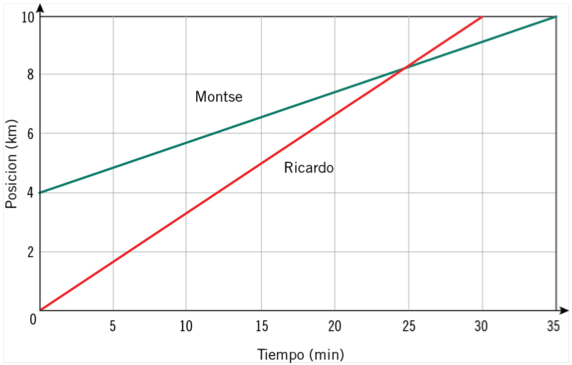
\includegraphics[width=\linewidth]{dist_tiempo_02}
                        \caption{La gráfica representa los viajes de Montse y Ricardo desde sus casa a la escuela.}
                        \label{fig:dist_tiempo_02}
                  \end{figure}

                  \begin{parts}
                        \part  ¿Qué distancia hay entre la casa de Montse y la escuela?

                        \begin{oneparchoices}
                              \choice 4 km
                              \CorrectChoice 6 km
                              \choice 8 km
                              \choice 10 km
                        \end{oneparchoices}

                        \part  ¿Cuánto se desplazó Ricardo para llegar a la escuela?

                        \begin{oneparchoices}
                              \choice 4 km
                              \choice 6 km
                              \choice 8 km
                              \CorrectChoice 10 km
                        \end{oneparchoices}


                        \part  ¿Qué tiempo le tomó llegar a Montse?

                        \begin{oneparchoices}
                              \choice 20 min.
                              \choice 25 min.\\
                              \choice 30 min.
                              \CorrectChoice 35 min.
                        \end{oneparchoices}

                        \columnbreak%

                        \part   ¿Qué tiempo hizo Ricardo?

                        \begin{oneparchoices}
                              \choice 20 min.
                              \choice 25 min.\\
                              \CorrectChoice 30 min.
                              \choice 35 min.
                        \end{oneparchoices}

                        \part  ¿Cuál fue la rapidez media de Montse durante su recorrido?

                        \begin{oneparchoices}
                              \choice 3.2 m/s
                              \choice 5.6 m/s \\
                              \CorrectChoice 2.86 m/s
                              \choice 2.68 m/s
                        \end{oneparchoices}

                        \part  ¿Cuál fue la rapidez media de Ricardo?

                        \begin{oneparchoices}
                              \choice 5.5 m/s
                              \choice 6.6 m/s\\
                              \CorrectChoice 5.6 m/s
                              \choice 6.5 m/s
                        \end{oneparchoices}

                        \part  ¿Quién llegó primero a la escuela?

                        \begin{oneparchoices}
                              \choice Montse.
                              \CorrectChoice Ricardo.\\
                              \choice Llegaron al mismo tiempo.\\
                              \choice No puede determinarse
                        \end{oneparchoices}




                        \part ¿Qué significa que sus gráficas se crucen?

                        \begin{choices}
                              \CorrectChoice Que Montse y Ricardo se encontraron 25 minutos después de que ambos partieron de sus casas.
                              \choice Que Montse y Ricardo viajaron con la misma rapidez durante su recorrido a la escuela.
                              \choice Que Montse y Ricardo tenían la misma velocidad después de 25 minutos de su recorrido.
                              \choice Ninguna de las anteriores.
                        \end{choices}


                  \end{parts}
            \end{multicols}
      }


      \question[5]{¿De qué longitud tendrá que ser el plano inclinado por utilizar si deseas
            subir un peso de 250 N a una altura de 5 m, si tu máxima capacidad te permite
            aplicar una fuerza de 50 N?

            \begin{solutionbox}{1.5cm}
            \end{solutionbox}
      }

      \question[6]{Un astronauta está en una estación espacial que se encuentra en órbita alrededor de la Tierra y por tanto en ausencia de la fuerza de gravedad. Alguien le pasa dos latas de comida cerradas y aparentemente idénticas. Sin embargo, una está completamente llena de alimento y la otra está vacía. ¿Cómo puede el astronauta distinguir cuál es la lata llena y cuál es la vacía sin abrirlas?}
      \begin{solutionbox}{1.5cm}
      \end{solutionbox}

      \newpage
      \question[8]{\include*{../questions/question034}}



      \question[8]{\include*{../questions/question029}}





\end{questions}
\end{document}